\chapter[][Sate of the Art]{State of the art}
\label{chap-biblio}

\section*{Introduction}

\section{Non-Uniform asymptotic methods}

There exist many different high-frequency approximations of the field echoed by the surfaces and interfaces of an inspected specimen. Some of these models lead to a discontinuous scattered field (which is not physical) and are therefore called non-uniform methods, as opposed to uniform models, which lead to continuous solutions.
\subsection{\acrfull{ge}}
The first approximation that can be applied to the study of wave propagation in a complex isotropic medium is the \acrfull{ge} model. It is a translation to elastodynamics of the geometrical optics theory. The field's propagation is described by ray tracing, each ray carrying a certain field value. At a given observation point, the field's value is the sum of the field values carried by each of the rays passing through this point. In the \acrshort{ge} theory, the incident, reflected and refracted rays are described. These rays are computed following Snell's laws of reflection and refraction :
\begin{equation}
    \frac{1}{c_{\alpha}}\cos\theta_{\alpha} = \frac{1}{c_{\beta}} \cos\theta_{\beta}
    \label{Snellrefl}
\end{equation}
In all this thesis, $\alpha=L,TH$ or $TV$ represents the type of the incident wave (\acrshort{L} for Longitudinal, \acrshort{TH} for Transverse Horizontal and \acrshort{TV} for Transverse Vertical) and $\beta$ is the type of the reflected, transmitted of diffracted wave.

When the incident wave meets a surface containing an edge, the propagation medium can be decomposed into four zones (see Fig.~\ref{illuzones}) :
\begin{itemize}
	\item Zone I : the incident rays are "shadowed" by the scattering surface and therefore do not illuminate this zone, called the shadow zone. The boundary between zones I and II is called the incident shadow boundary.
    \item Zone II : only the incident rays propagate in this zone.
    \item Zone III :  the incident rays are reflected by the scattering surface and mode occurs. This zone is illuminated by the incident rays and by the mode-converted reflected rays.
    \item Zone IV : the incident rays are reflected and mode conversion may occur. This zone is illuminated by incident rays and by L and T reflected waves.
\end{itemize}
The boundaries separating each of these zones are called the shadow boundaries. In the case where there is no mode conversion (determined by Snell's law of reflection \eqref{Snellrefl}), there is no Zone III. 

The displacement fields carried by the reflected and refracted rays are proportional to the field incident of the reflecting or refracting interfaces. This proportionality is contained in multiplicative coefficient called reflection or transmission coefficients respectively, which depend on the properties of the propagation medium and on the directions of incidence and observation.

In reality, part of the scattered wave propagates in Zone I. Indeed, part of the incident wave arrives on the edge and is diffracted. This diffracted wave propagates in all directions. The \acrshort{ge} model does not account for the diffracted wave, as they can not be predicted by ray tracing. To complete the \acrshort{ge} model, Keller \cite{GTD} has developed the \acrfull{gtd}.

\begin{figure}
    \centering
    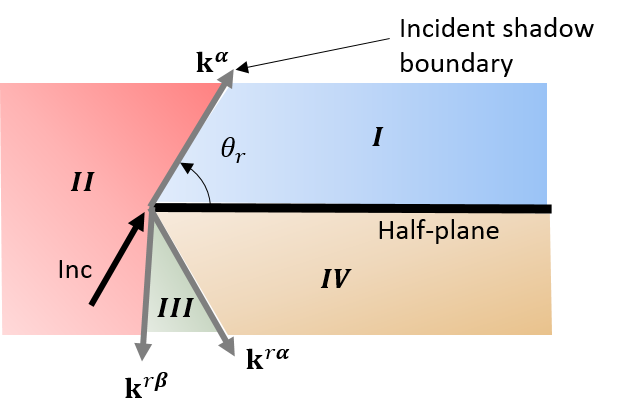
\includegraphics[height=0.33\textheight]{images/chapter1/ShadowBoundary.png}
    \caption{Incident wave on an edge}
    \label{illuzones}
\end{figure}

\subsection{\acrfull{gtd}}
\label{C1:GTD}
The \acrfull{gtd} was initially developed by Keller \cite{GTD} for optical waves and adapted to elastodynamics by Achenbach and Gautesen \cite{AchenbachGautesen, Achenbach}. This theory postulates the existence of diffracted waves emanating from the edge of the scattering surface. A incident ray on an edge generates a cone of rays, called Keller's cone of diffraction \cite{GTD}, represented on Fig.~\ref{KellerCone}. The cone's principal axis is the diffracting edge, its principal angle $\Omega_{\beta}$ is determined by Snell's law of diffraction :
\begin{equation}
    \frac{1}{c_{\alpha}}\cos\Omega_{\alpha} = \frac{1}{c_{\beta}} \cos\Omega_{\beta}
\end{equation}

\begin{figure}
    \centering
    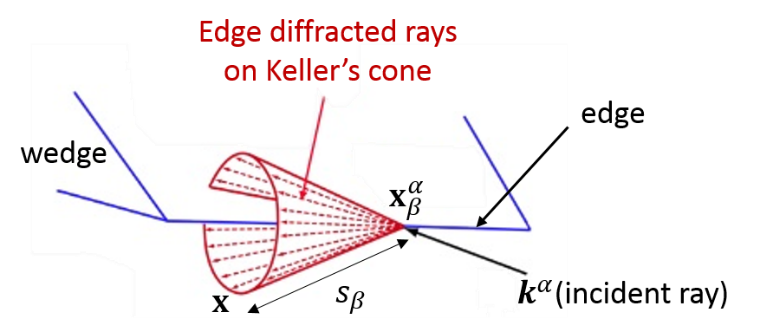
\includegraphics[width=\textwidth]{images/chapter1/KellerCone.png}
    \caption{Diffracted rays generated by an incident ray}
    \label{KellerCone}
\end{figure}
where $\Omega_{\alpha}$ is the angle between the incident wave vector $\mathbf{k}^{\alpha}$ and the diffracting edge. In this chapter, the bold font is used to denote vectors. Rahmat-Samii \cite{ConePhoto} has observed this cone in a hotel room, see Fig.~\ref{PhotoCone}. A ray of light is incident on the corner of a table and generates a cone of diffracted rays, whose intersection with the door is a circle.

\begin{figure}
    \centering
    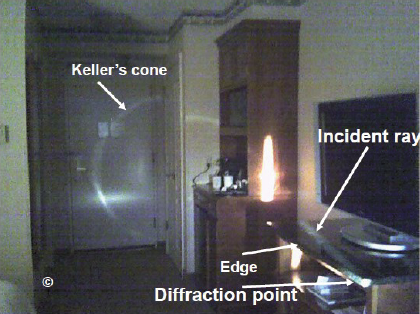
\includegraphics{images/chapter1/HotelCone.png}
    \caption{Observation of Keller's cone of diffraction}
    \label{PhotoCone}
\end{figure}

\acrshort{gtd} is also a ray tracing method, meaning that at a given observation point $\mathbf{x}$, the total field $\mathbf{u^{tot}}$ is the sum of the fields carried by each ray passing through $\mathbf{x}$ :
\begin{equation}
    \mathbf{u}^{tot}(\mathbf{x})=\mathbf{u}^{(GE)}(\mathbf{x})+\sum_{\beta} \mathbf{u}^{diff}_{\beta}(\mathbf{x})
    \label{GTDtot}
\end{equation}
where $\mathbf{u^{(GE)}}$ is the \acrshort{ge} displacement field, composed of the incident, reflected and refracted fields and $\mathbf{u^{diff}_{\beta}}$ is the diffracted field of type $\beta=L,TH,TV$. The diffracted field's amplitude decreases as the distance $r$ from the point of impact $\mathbf{x}_{\beta}^{\alpha}$ of the incident wave on the diffracting edge grows. As for the \acrshort{ge} field, the diffracted field is proportional to the field incident on the edge. This proportionality is characterized by a multiplicative coefficient called the diffraction coefficient, which depends on the propagation medium, on the geometry of the diffracting object and on the direction of observation. This is summarized by the following equation :
\begin{equation}
    \mathbf{u}_{\beta}^{diff}(\mathbf{x})=u_{\alpha}(x_{\beta}^{\alpha})D_{\beta}^{\alpha}(\theta)\dfrac{e^{ik_{\beta}S_{\beta}}}{\sqrt{k_{\beta}R_{\beta}^{diff}}}\mathbf{e_{\beta}}(\mathbf{x})
\end{equation}
where $u_{\alpha}$ is the scalar value of the incident field, $D_{\beta}^{\alpha}$ is the diffraction coefficient, $\theta$ is the direction of observation, $k_{\beta}$ is the diffracted wave's wave number, $S_{\beta}$ is the distance between the observation point $\mathbf{x}$ and the diffraction point $\mathbf{x}_{\beta}^{\alpha}$ (visible Fig.~\ref{KellerCone}), $\mathbf{e_{\beta}}(M)$ is the unit polarization vector of the diffracted wave at point $\mathbf{x}$ and $R_{\beta}^{diff}$ is a distance parameter which will be computed later, at section \ref{}.

This principle is called the locality principle, because it stipulates that the value of the field at any given point is fully determined by the field in the close vicinity of the point from which the ray carrying this field emanates. Computation of diffracted fields can therefore be reduced to a number of canonical problems, such as diffraction by a tip or a half plane. In the present thesis, the canonical problem of interest is diffraction by a wedge.

\acrshort{gtd} is a high-frequency model which accounts for edge-diffracted waves. However, the resulting field is discontinuous at shadow boundaries and the diffraction coefficient possesses poles in the directions of specular reflection, rendering the diffracted field divergent in these directions. It is therefore not physical. Some uniform corrections have been proposed to solve this problem, resulting in continuous fields. They are presented in the following. 

\section{Uniform corrections}

\subsection{\acrfull{ka}}
The \acrfull{ka}, also called \acrfull{po} was first developed in optics by Baker and Copson \cite{POoptics} before being extended to acoustic and electromagnetic waves \cite{POtechreport, POLewis} before being adapted by Chapman to elastic waves \cite{POChapman}, where it is essentially used for \acrshort{ndt} applications \cite{Schmerr,Dorval}.

The Kirchoff Approximation is a high frequency approximation for which the scattering surface is assumed to behave locally like a plane. This means that for each point of the surface, the plane tangent to the surface at that point is determined and the displacement field on the illuminated side is computed using \acrshort{ge}. The other side of the plane is shadowed and the total displacement field vanishes. The jump in the displacement between both sides of this plane is called \acrfull{cod} and noted $\lbrack \mathbf{u}(\mathbf{x}) \rbrack$. It appears in an integral formulation of the scattered field, called the Rayleigh-Sommerfeld integral \cite{POChapman} :
\begin{equation}
u_p(\mathbf{x})=\int_{S^+}\lbrack u_i(\mathbf{x'})G_{ij}^{(p)}(\mathbf{x},\mathbf{x'})n_j(\mathbf{x'})\,d^2\mathbf{x'}
\label{intKA}
\end{equation}
where $u_p$ is the $p$-th coordinate of the displacement scattered field, $s^+$ is the lit side of the scattering surface, $n$ is the outward normal to $S^+$ and $G_{ij}^{(p)}(\mathbf{x},\mathbf{x'})$ is the $(ij)$ component of Green's stress tensor $G^{(p)}(\mathbf{x},\mathbf{x'})$, which is the stress produced at $\mathbf{x}$ by a unit traction acting along the $p$-axis at point $\mathbf{x'}$ on $S^+$, its expression is given in \cite{POChapman}. In this integral, the Green's tensor is therefore used to propagate the local solution $\lbrack \mathbf{u}(\mathbf{x'}) \rbrack$ to the whole propagation domain.

The \acrshort{ka} scattered field models diffraction as well as reflection and is continuous in the whole space. comparisons between \acrshort{ka}, \acrshort{gtd} and the exact solution have been made for a strip-like crack illuminated by a transversal wave \cite{POChapman,systmodel}. The Kirchhoff Approximation gives good results close to the specular reflections, as can be expected since the model is based on the \acrshort{ge} field. However, further away from these regions, it is inaccurate, as opposed to the \acrshort{gtd} which models diffraction correctly.

The \acrshort{gtd} solution models diffraction well is non-uniform in the sense that it diverges at shadow boundaries. The \acrshort{ka} on the other hand, is uniform but doesn't model diffraction correctly. Furthermore, it requires meshing of the scattering surface. To overcome inaccuracies of the \acrshort{gtd} and \acrshort{ka} models, an other model has been developed, called the \acrfull{ptd}.

\subsection{\acrfull{ptd}}
The \acrfull{ptd} was first developed for acoustic and electromagnetic waves by Ufmitsev \cite{Ufmi} and was extended to elastodynamics by Darmon et al. \cite{DarmonKA}. The idea is to combine \acrshort{gtd} and \acrshort{ka} models to overcome their shortcomings. This is done by adding a corrective term to the \acrshort{ka} diffracted field which is the difference between the \acrshort{gtd} and the \acrshort{ka} diffracted fields :
\begin{equation}
\mathbf{u}^{tot (PTD)}=\mathbf{u}_{\alpha}(\mathbf{x})+\mathbf{u}^{sc (PTD)}(\mathbf{x})
\end{equation}
where $\mathbf{u}_{\alpha}$ is the incident field and
\begin{equation}
\mathbf{u}^{sc (PTD)}(\mathbf{x})=\sum_{\beta}\left[\mathbf{u}^{\alpha(KA)}_{\beta}(\mathbf{x})+u_{\alpha}(\mathbf{x}_{\beta}^{\alpha})\left(D_{\beta}^{\alpha(GTD)}(\mathbf{x})-D_{\beta}^{\alpha(KA)}(\mathbf{x})\right)\dfrac{e^{ik_{\beta}S_{\beta}}}{\sqrt{k_{\beta}R_{\beta}^{diff}}}\right]
\label{eqPTD}
\end{equation}
where  $\mathbf{u}^{\alpha(KA)}_{\beta}$ is obtained by \eqref{intKA}, $D_{\beta}^{\alpha(GTD)}$ is the \acrshort{gtd} diffraction coefficient and $D_{\beta}^{\alpha(KA)}$ is the \acrshort{ka} diffraction coefficient obtained by an asymptotic evaluation of \eqref{intKA}, for $k_{\beta}S_{\beta}>>1$ (see appendix \ref{PhaseStationnaire}), which correspond to the contribution of the scattering edges to the Rayleigh-Sommerfeld integral. In the far-field, the \acrshort{ka} diffraction coefficient diverges at specular directions, compensating the divergence of the \acrshort{gtd} diffraction coefficient. The diffracted field then disappears, leaving only the Kirchhoff evaluation, which is accurate in regions of specular reflection.

Far from the incident and specular directions, we have :
\begin{equation}
\mathbf{u}_{\beta}^{\alpha(KA)}(\mathbf{x})\approx \mathbf{u}_{\beta}^{diff(KA)}(\mathbf{x}) \approx u_{\alpha}(\mathbf{x}_{\beta}^{\alpha})D_{\beta}^{\alpha(KA)}(\mathbf{x})\dfrac{e^{ik_{\beta}S_{\beta}}}{\sqrt{k_{\beta}R_{\beta}^{diff}}}
\end{equation}
Substituting this into \eqref{eqPTD}, we find that in these regions, the \acrshort{ka} contribution vanishes and only the \acrshort{gtd} field remains, which models diffraction accurately.

The Physical theory of diffraction has been developed in the \acrshort{ndt} software platform CIVA \cite{systmodel}. It provides a good description of the scattered field in the directions of specular reflection, as well as far from the shadow boundaries. However, it requires meshing of the scattering surface for the \acrshort{ka} model as well as meshing of the flaw contour for the \acrshort{gtd} model. Another uniform model has been developed, called the \acrfull{uat}.

\subsection{\acrfull{uat}}
The \acrfull{uat} was first developed in for acoustics and electromagnetics by Lewis and Boersma \cite{Lewis} in two dimensions and was extended to three-dimensional problems by Ahluwalia \cite{Ahluwalia} and to a curved wedge by Lee and Deschamps \cite{LeeDeschamps} before being extended to elastodynamics by Achenbach et al. \cite{Achenbach}. It is a correction of the \acrshort{gtd} model where the \acrshort{ge} field is modified to compensate the divergence in the \acrshort{gtd} field and smooth the discontinuity in the \acrshort{ge} field. The total field \eqref{GTDtot} becomes :
\begin{equation}
\mathbf{u}^{tot(UAT)}(\mathbf{x})=\left[ \overline{F}(\xi_{\alpha})-\hat{\overline{F}}(\xi_{\alpha})\right]\mathbf{u}_{\alpha}(\mathbf{x})+\sum_{\beta} \left[ \overline{F}(\xi_{\beta})-\hat{\overline{F}}(\xi_{\beta})\right]\mathbf{u}^{ref}_{\beta}(\mathbf{x})+\mathbf{u}_{\beta}^{diff(GTD)}(\mathbf{x})
\label{eqUAT}
\end{equation}
where $\overline{F}$ is the Fresnel function, defined by 
\begin{equation}
\overline{F}(X)=\frac{1}{\sqrt{i\pi}}\int_X^{+\infty} e^{it^2}\,dt
\label{defFresnel}
\end{equation}
and 
\begin{equation}
\hat{\overline{F}}(X)=e^{i\frac{\pi}{4}}\dfrac{e^{iX^2}}{2X\sqrt{\pi}}
\end{equation}
$\mathbf{u}^{ref}_{\beta}$ is the reflected field of type $\beta$, $\mathbf{u}_{\beta}^{diff(GTD)}$ is the \acrshort{gtd} diffracted field of type $\beta$ and $\xi_{\alpha}$ and $\xi_{\beta}$ are detour parameters defined in \cite{LeeDeschamps}. They evaluate the proximity of the observation point to the shadow boundary of the incident wave for $\xi_{\alpha}$ and of the reflected wave for $\xi_{\beta}$. The presence of the Fresnel function $\overline{F}$ smooths the discontinuity in the \acrshort{ge} field while the function $\hat{\overline{F}}$ compensates the divergence of the \acrshort{gtd} diffracted field. Therefore, the total \acrshort{uat} field is spatially uniform.

In \eqref{eqUAT} the incident and reflected fields are defined in the the whole space, this means in particular that they must be extended to their shadow zones. This is achieved by constructing the fictitious rays in the shadow zones \cite{Bouche,Molinet}, see Fig.~\ref{FictRays}. This makes \acrshort{uat} difficult to implement for complex geometries. A uniform model which is simpler to implement, the \acrfull{utd} has therefore been developed.

\begin{figure}[h]
    \centering
    \begin{subfigure}[b]{0.45\textwidth}
        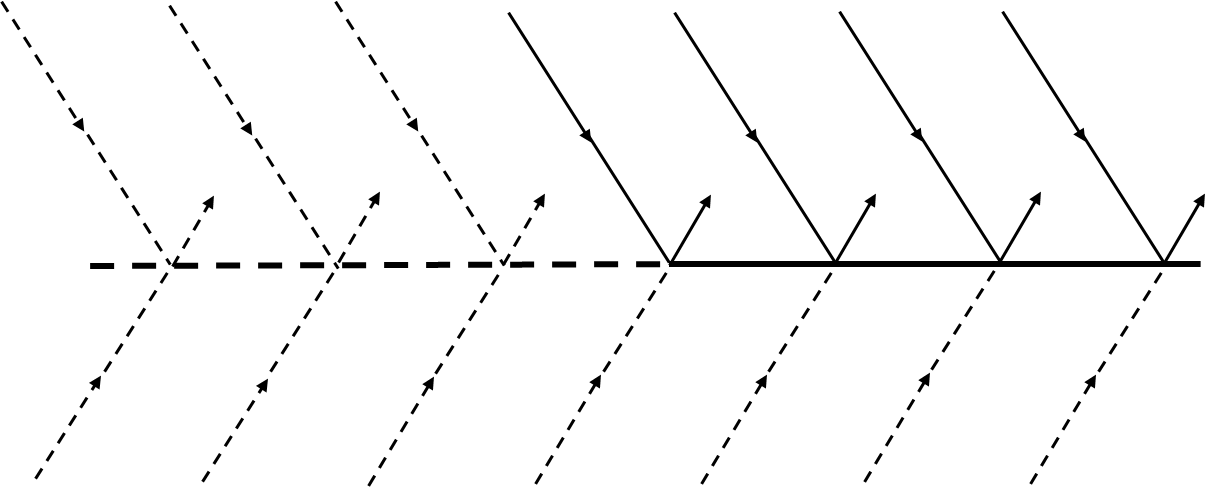
\includegraphics[width=\textwidth]{images/chapter1/FictitiousStraight.png}
        \caption{Fictitious rays constructed in the case of a straight scatterer}
        \label{Straightfict}
    \end{subfigure}
    ~ 
    \begin{subfigure}[b]{0.45\textwidth}
        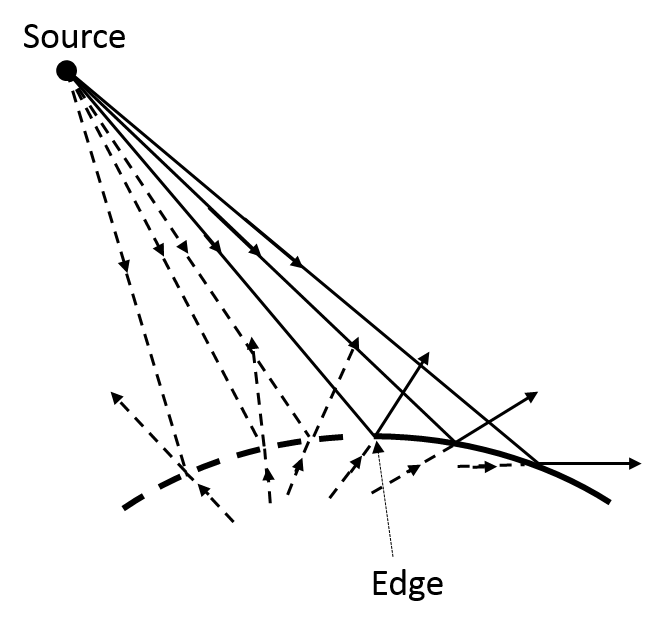
\includegraphics[width=\textwidth]{images/chapter1/FictitiousCurved.png}
        \caption{Fictitious rays constructed in the case of a curved scatterer}
        \label{Curvedfict}
    \end{subfigure}
    \caption{(Reproduced from \cite{Bouche,Molinet}) Extension of the reflected field to its shadow zone using fictitious rays. Dashed thick lines are extensions of the scatterers beyond the crack edge and dashed thin lines are incident and fictitious reflected rays on these extensions.}
    \label{FictRays}
\end{figure}

\subsection{\acrfull{utd}}
The \acrfull{utd} was initially developed for acoustic and electromagnetic waves by Kouyoumjian and Pathak \cite{Kouyoumjian,PathakKouyou} and was extended to elastodynamics by Kamta-Djakou during her PhD thesis \cite{Audrey,AKDthese}. This method consists of correcting the \acrshort{gtd} diffraction coefficient using a transition function $F$. For the problem of diffraction by a wedge of angle $\varphi$, this is expressed as :
\begin{equation}
    D_{\beta}^{\alpha(UTD)}(\zeta,\theta)=(-1)^{M_{\beta}+1}D_{\beta}^{\alpha(GTD)}(\theta)\left[ \sum_{j=1}^{M_{\beta}} F(\zeta a^j_{\beta})\prod_{\underset{k\neq j}{k=1}}^{M_{\beta}} \dfrac{s_\beta^{k}}{(s_\beta^{j}-s_\beta^{k})}\right]
    \label{DUTDGTD}
\end{equation}
where $\beta=L,TH,TV$ is the type of the diffracted wave, $\theta$ is the observation angle, $(\lambda^j_{\beta}), 1\leq j\leq M_{\beta}$ are the poles of the diffraction coefficient mentioned in section \ref{C1:GTD} (methods of computation of these poles will be given in the following chapters) and 
\begin{equation}
    a_{\beta}^j=-i(s_{\beta}^j)^2=2\cos^2\left(\frac{\lambda_{\beta}^j-\theta+\varphi/2}{2}\right)
\end{equation}
$\zeta$ is a far-field parameter which can be defined as
\begin{equation}
    \zeta=k_{\beta}\left(\dfrac{R_{\beta}^{diff}}{R_{\beta}^{GE}}\right)^2
\end{equation}
where $R_{\beta}^{diff}$ is the divergence factor of the diffracted wave and $R_{\beta}^{GE}$ is the divergence factor of reflected waves, both of these will be computed at section \ref{}. Finally, $F$ is a transition function defined as the complex conjugate of the Kouyoumjian function \cite{Kouyoumjian}
\begin{equation}
    F(X)=-2i\sqrt{i\pi X}e^{-iX}\overline{F}(\sqrt{X})
\end{equation}
$\overline{F}$ is the Fresnel function defined by \eqref{defFresnel}.

Far from the shadow boundaries, $\zeta a_{\beta}^j >>1$ and
\begin{equation}
F(\zeta a_{\beta}^j) \rightarrow 1 \mbox{ and } (-1)^{M_{\beta}+1}\left[ \sum_{j=1}^{M_{\beta}} \prod_{\underset{k\neq j}{k=1}}^{M_{\beta}} \dfrac{s_\beta^{k}}{(s_\beta^{j}-s_\beta^{k})}\right]=1
\end{equation}
In this case, the \acrshort{utd} solution for the diffracted field is the same as the \acrshort{gtd} diffracted field. Close to the shadow boundaries, Kamta-Djakou \cite{AKDthese} has shown that the transition functions makes the diffracted field discontinuous when crossing shadow boundaries and that these irregularities compensate exactly those of the \acrshort{ge} field, so that the total field computed using \eqref{GTDtot} is uniform.

The \acrfull{utd} has been validated numerically in far-field configurations in \cite{AKDthese}. It models the diffracted field well and provides a spatially uniform solution while being simple to implement.

The \acrshort{ptd}, \acrshort{uat} and \acrshort{utd} methods presented are all uniform \textit{corrections} of the \acrshort{gtd} field. This means that they all rely on a preexisting \acrshort{gtd} solution, which must therefore be accurate. In the following, the two main existing \acrshort{gtd} approaches to the problem of diffraction of an elastic wave by a stress-free wedge are presented.

\section{Principal \acrshort{gtd} elastic wedge diffraction models}

\begin{figure}
\centering
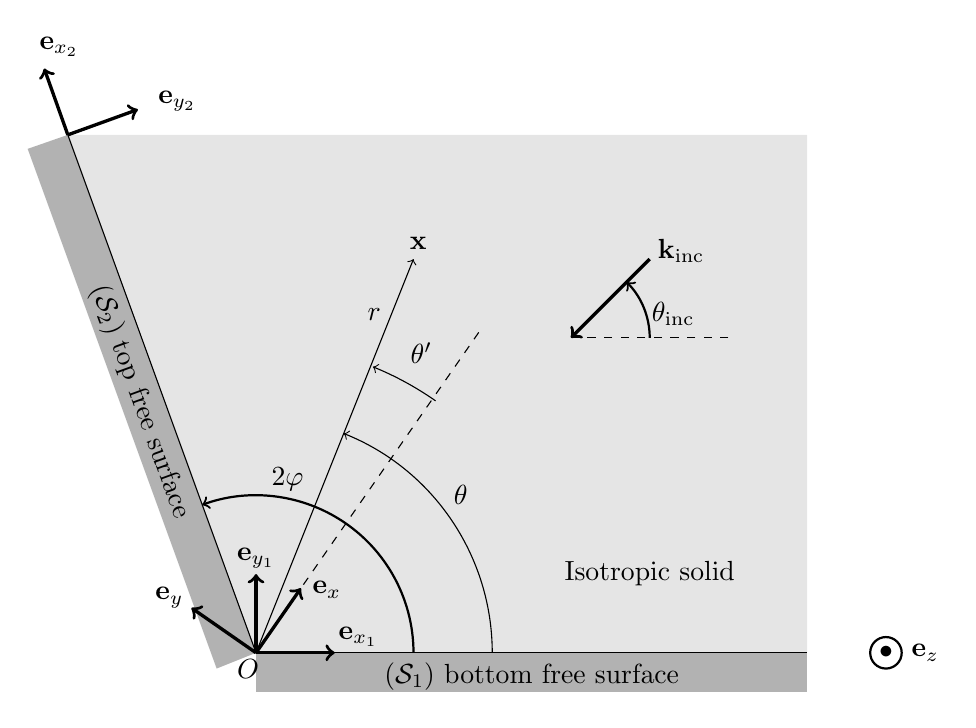
\begin{tikzpicture}
\fill[color=gray!20] (0,0) -- (7,0)  -- (7,6.5778) -- (-2.39,6.5778) -- cycle;  
\draw[ thick, ->] (2,0) arc (0:110:2);

\fill[color=gray!60] (0,0) -- (7,0)  -- (7,-0.5) -- (0,-0.5) -- cycle;  

\fill[color=gray!60] (0,0) --  (-2.39,6.5778) --(-2.9,6.4) -- (-0.5,-0.2) -- cycle; 


\draw[color = black]  (0,0) -- (7,0) node[midway,below] {($\mathcal{S}_1$) bottom free surface};

\draw[color = black]  (0,0) -- (-2.39,6.5778) node[midway,below,sloped] { ($\mathcal{S}_2$) top free surface};

\draw[very thick, ->] (-2.39,6.5778) -- (-2.69,7.42);

\node[scale=1] at (-2.5,7.7){ $\mathbf{e}_{x_2}$};

\draw[very thick, ->] (-2.39,6.5778) -- (-1.5,6.9);

\node at (-1,7){$\mathbf{e}_{y_2} $};


\node at (0.4,2.2){$2 \varphi$} ; 

\draw[very thick, ->] (0,0) -- (1,0);

\node at (1.3,0.2) {$\mathbf{e}_{x_1} $};

\draw[very thick, ->] (0,0) -- (0,1);

\node at (0,1.2){$\mathbf{e}_{y_1} $};

\node at (8,0) {$\bullet$};

\draw[thick] (8,0) circle (0.2);

\node at (8.5,0){$\mathbf{e}_{z}$};

\draw[very thick, ->] (0,0) -- (0.57,0.82);

\node at (0.9,0.8){$\mathbf{e}_x$};

\draw[very thick, ->] (0,0) -- (-0.82, 0.57);

\node at (-1.1,0.7){$\mathbf{e}_y$};

\draw[very thick, ->] (5,5) -- (4,4);

\draw[dashed] (6,4) -- (4,4);

\draw[ thick, ->] (5,4) arc (0:45:1);

\node at (5.3,4.3){$\theta_{\rm inc}$};

\node at (5.4,5.1){$\mathbf{k}_{\rm inc}$};

\node at (-0.1,-0.2){$O$};

\node at (5,1){Isotropic solid};

% point observation

\draw[->] (0,0) -- (2,5); 

\draw[->] (3,0) arc (0:68.2:3);

\draw[dashed] (0,0) -- (2.85,4.1);

\node at (2.6,2){$\theta$};

\node at (1.5,4.3){$r$};

\node at (2.06,5.2){$\mathbf{x}$};

\draw[->] (2.28,3.2) arc (55:68:4);

\node at (2.1,3.8){$\theta'$};

\end{tikzpicture}
\caption{Stress-free wedge of angle $2\varphi$ illuminated by a plane wave of wave vector $\mathbf{k}^{\rm inc}$. The dotted line is the wedge bisector.}
\label{C1:wedge}
\end{figure}

As seen in the previous section, an accurate uniform scattering model requires a trust-worthy initial \acrshort{gtd} solution in order to be developed. The aim of this thesis will therefore be to develop a generic and trust-worthy wedge diffraction \acrshort{gtd} model. To our knowledge, there is no fully analytical resolution of the problem of elastic wedge diffraction available in scientific literature, and the preferred approach is semi-analytical. We begin this work by a review of the two main existing 2D wedge-diffraction models. These two models have been presented and compared by Gautesen and Fradkin \cite{GautesenFradkin}, who also discuss their numerical validation. Experimental validation  of these codes has been done by Chapman et al. \cite{ChapmanLTval}.

The geometry of the problem is visible in Fig.~\ref{C1:wedge}. A stress-free wedge of angle $2\varphi<\pi$ is illuminated by a a plane wave of which forms an angle $\theta_{inc}$ with the bottom face of the wedge. The problem is two-dimensional in the sense that the incident wave vector is in the plane normal to wedge edge. In all the following, the harmonic time-dependency factor $e^{i\omega t}$ (where $\omega$ is the circular frequency and $t$ is time) will be omitted. $(0;\mathbf{e}_{x_1},\mathbf{e}_{y_1},\mathbf{e}_z)$ is the orthonormal basis of a Cartesian coordinate system where the $z$-axis coincides with the wedge edge and the $x_1$ axis coincides with the bottom face of the wedge. The polar coordinates associated to the system are $\mathbf{x}=(r,\theta)$ In this coordinate system, the incident wave vector is :
\begin{equation}
\mathbf{k}^{inc}=-(\cos\theta_{inc},\sin\theta_{inc})_{(\mathbf{e}_{x_1},\mathbf{e}_{y_1})}
\end{equation}
$(0;\mathbf{e}_x,\mathbf{e}_y,\mathbf{e}_z)$ is the orthonormal basis of a Cartesian coordinate system where the $x$-axis coincides with the wedge bisector and the polar coordinates associated to the system are $\mathbf{x}=(r,\theta')$.

In both of the following approaches, the the symmetry of the problem with respect to the wedge bisector is used and the problem is split in two : a symmetric problem and an antisymmetric problem.


\subsection{The \acrfull{si} Method}
\subsection{The \acrfull{lt} Method}